% Copyright 2004 by Till Tantau <tantau@users.sourceforge.net>.
%
% In principle, this file can be redistributed and/or modified under
% the terms of the GNU Public License, version 2.
%
% However, this file is supposed to be a template to be modified
% for your own needs. For this reason, if you use this file as a
% template and not specifically distribute it as part of a another
% package/program, I grant the extra permission to freely copy and
% modify this file as you see fit and even to delete this copyright
% notice. 

\documentclass{beamer}

% There are many different themes available for Beamer. A comprehensive
% list with examples is given here:
% http://deic.uab.es/~iblanes/beamer_gallery/index_by_theme.html
% You can uncomment the themes below if you would like to use a different
% one:
%\usetheme{AnnArbor}
%\usetheme{Antibes}
%\usetheme{Bergen}
%\usetheme{Berkeley}
%\usetheme{Berlin}
%\usetheme{Boadilla}
%\usetheme{boxes}
%\usetheme{CambridgeUS}
%\usetheme{Copenhagen}
%\usetheme{Darmstadt}
%\usetheme{default}
%\usetheme{Frankfurt}
%\usetheme{Goettingen}
%\usetheme{Hannover}
%\usetheme{Ilmenau}
%\usetheme{JuanLesPins}
%\usetheme{Luebeck}
\usetheme{Madrid}
%\usetheme{Malmoe}
%\usetheme{Marburg}
%\usetheme{Montpellier}
%\usetheme{PaloAlto}
%\usetheme{Pittsburgh}
%\usetheme{Rochester}
%\usetheme{Singapore}
%\usetheme{Szeged}
%\usetheme{Warsaw}


% Customize Warsaw color 
\setbeamercolor*{palette primary}{use=structure,fg=white,bg=red!50!black}
\setbeamercolor*{palette secondary}{use=structure,fg=white,bg=red!60!black}
\setbeamercolor*{palette tertiary}{use=structure,fg=white,bg=red!70!black}

% Customize Warsaw block title and background colors
\setbeamercolor{block title}{bg=red!50!black,fg=white}


% List your packages here

\usepackage[colorinlistoftodos]{todonotes}


\title[Progress Update]{A General Open Source Platform for Building Energy Management}

% % A subtitle is optional and this may be deleted
% \subtitle{Product Proposal}

\author[B.~Lauer]{Brian~Lauer\\\and
Advisor: Dr. Suruz Miah}
% - Give the names in the same order as the appear in the paper.
% - Use the \inst{?} command only if the authors have different
%   affiliation.

\institute[Bradley University] % (optional, but mostly needed)
{
  Department of Electrical and Computer Engineering\\
  Bradley University\\
  1501 W. Bradley Avenue\\
  Peoria, IL, 61625, USA
}
% - Use the \inst command only if there are several affiliations.
% - Keep it simple, no one is interested in your street address.

\date[Friday~17,~2020]{Friday, April~17,~2020}
% - Either use conference name or its abbreviation.
% - Not really informative to the audience, more for people (including
%   yourself) who are reading the slides online

\logo{\hfill\href{http://www.bradley.edu}{
\includegraphics[width=0.75cm]{../figs/logoBU1-Print}}}  % place logo in every page 


\subject{Mobile Robot Localization}
% This is only inserted into the PDF information catalog. Can be left
% out. 

% If you have a file called "university-logo-filename.xxx", where xxx
% is a graphic format that can be processed by latex or pdflatex,
% resp., then you can add a logo as follows:

% \pgfdeclareimage[height=0.5cm]{university-logo}{university-logo-filename}
% \logo{\pgfuseimage{university-logo}}

% Delete this, if you do not want the table of contents to pop up at
% the beginning of each subsection:

% Let's get started
\begin{document}

\begin{frame}
  \titlepage
\end{frame}

\begin{frame}{Outline}
  \tableofcontents
  % You might wish to add the option [pausesections]
\end{frame}


\section{Introduction}
\begin{frame}{Introduction}
\begin{figure}
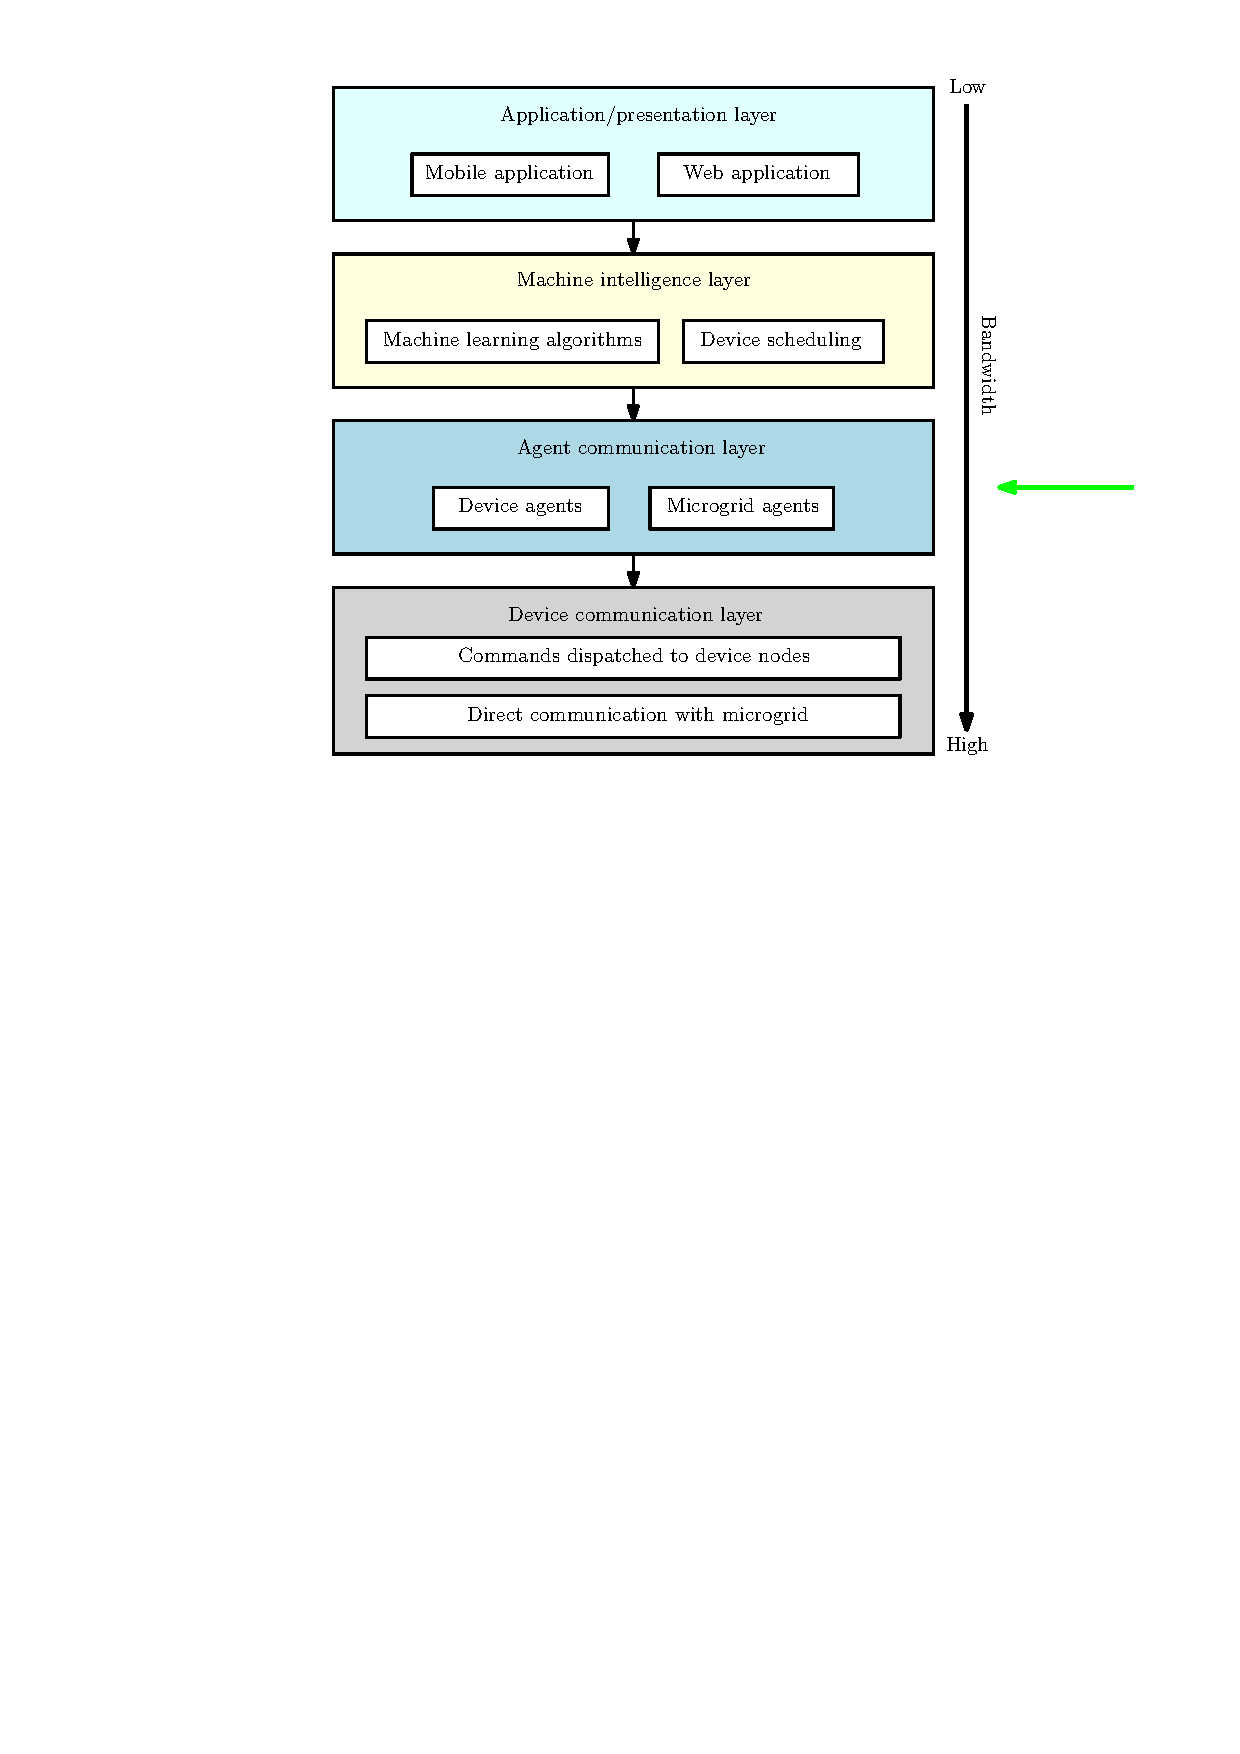
\includegraphics[scale=0.43]{../figs/ipe/BEMS-softwareArchitectureAgents}
\caption{High level software architecture, currently working on determining and developing agents}
\end{figure}
\end{frame}

\section{Progress}
\begin{frame}{Progress}
\begin{itemize}
\item Fixed problem with login form not sending a HTTP POST request, had to add \texttt{method="post"} attribute to \texttt{form} element
\item Began work on integrating SQLite3 database into web application, may switch to MySQL, PostgreSQL
\item Created class \texttt{DatabaseConnection} for connecting to the database and closing the connection 
\item Create github repo at \texttt{https://github.com/blauer890/NewBEMS}
\end{itemize}
\end{frame}

\begin{frame}{Progress}
Rough plan for development
\begin{enumerate}
\item Agent platform
\item Device APIs (only WeMo switch for now)
\item Microgrid simulation
\item Flask app development
\item User interface development
\end{enumerate}
Other steps will be added as development goes on
\end{frame}

\section{Agent Platform}
\begin{frame}{Agent Platform}
\begin{itemize}
\item Agent definition - autonomous software entity that is able to interact with its environment and other agents
\item In platform, Python classes will represent agents with methods representing their corresponding behavior
\item Requires view functions in flask applications to be able to publish messages to a central bus
\end{itemize}
\end{frame}

\begin{frame}{Agent Platform}
\begin{block}{Agents Planned}
\begin{itemize}
\item \texttt{DeviceAgent} - can control and monitor devices on the network, for now will only be WeMo switch
\item \texttt{DiscoveryAgent} - detecting devices on the network through their APIs
\item \texttt{MicrogridAgent} - report on current state of the simulated microgrid, will require some research to determine how to build this application
\item \texttt{MetadataAgent} - will accept SQL queries from agents and run them
\item \texttt{NotificationAgent} - send necessary notifications to a user through either SMS or email
\item \texttt{RealtimeAgent} - allows agents to submit queries or publish data to a database storing time data
\end{itemize}
\end{block}
\end{frame}

\section{Objectives}

\begin{frame}{Objectives}
\begin{itemize}
\item Determine libraries to for building the message passing system
\item Start writing agents
\item Build WeMo API
\end{itemize}
\end{frame}
% All of the following is optional and typically not needed. 
\appendix
\section<presentation>*{\appendixname}
\subsection<presentation>*{For Further Reading}

\begin{frame}[allowframebreaks]
  \frametitle<presentation>{For Further Reading}
    
  \begin{thebibliography}{10}
    
  \setbeamertemplate{bibliography item}[online]
  
  \bibitem{BEMOSSWiki}
  BEMOSS Agent Background Wiki
  \newblock Agent Background page
  \newblock \texttt{https://github.com/bemoss/BEMOSS3.5/
  wiki/Agent-Background}
  
  \bibitem{Spadedocs}
  SPADE Read the Docs
  \newblock SPADE documentation
  \newblock \texttt{https://spade-mas.readthedocs.io/en/latest/readme.html}
  \end{thebibliography}
\end{frame}

\end{document}



%%% Local Variables:
%%% mode: latex
%%% TeX-master: t
%%% End:
